
% Быть посвободнее при склеивании слов
\sloppy

% Настройка листингов
\renewcommand{\lstlistingname}{Листинг}
\lstset{
	frame=single, % adds a frame around the code
	rulesepcolor=\color{gray},
	rulecolor=\color{black},
	breaklines=true,
	xleftmargin=2em,
	extendedchars={true},
	inputencoding={utf8},
	basicstyle={\ttfamily \scriptsize},
	keywordstyle={\rmfamily \bfseries},
	commentstyle={\rmfamily \itshape},
	tabsize={2},
	numbers={left},
	frame={single},
	showstringspaces={false},
}
\lstdefinestyle{java}{
	breaklines={true},
	texcl=true,
	language={Java},
}
\lstset{
    literate={а}{{\selectfont\char224}}1
    {б}{{\selectfont\char225}}1
    {в}{{\selectfont\char226}}1
    {г}{{\selectfont\char227}}1
    {д}{{\selectfont\char228}}1
    {е}{{\selectfont\char229}}1
    {ё}{{\"e}}1
    {ж}{{\selectfont\char230}}1
    {з}{{\selectfont\char231}}1
    {и}{{\selectfont\char232}}1
    {й}{{\selectfont\char233}}1
    {к}{{\selectfont\char234}}1
    {л}{{\selectfont\char235}}1
    {м}{{\selectfont\char236}}1
    {н}{{\selectfont\char237}}1
    {о}{{\selectfont\char238}}1
    {п}{{\selectfont\char239}}1
    {р}{{\selectfont\char240}}1
    {с}{{\selectfont\char241}}1
    {т}{{\selectfont\char242}}1
    {у}{{\selectfont\char243}}1
    {ф}{{\selectfont\char244}}1
    {х}{{\selectfont\char245}}1
    {ц}{{\selectfont\char246}}1
    {ч}{{\selectfont\char247}}1
    {ш}{{\selectfont\char248}}1
    {щ}{{\selectfont\char249}}1
    {ъ}{{\selectfont\char250}}1
    {ы}{{\selectfont\char251}}1
    {ь}{{\selectfont\char252}}1
    {э}{{\selectfont\char253}}1
    {ю}{{\selectfont\char254}}1
    {я}{{\selectfont\char255}}1
    {А}{{\selectfont\char192}}1
    {Б}{{\selectfont\char193}}1
    {В}{{\selectfont\char194}}1
    {Г}{{\selectfont\char195}}1
    {Д}{{\selectfont\char196}}1
    {Е}{{\selectfont\char197}}1
    {Ё}{{\"E}}1
    {Ж}{{\selectfont\char198}}1
    {З}{{\selectfont\char199}}1
    {И}{{\selectfont\char200}}1
    {Й}{{\selectfont\char201}}1
    {К}{{\selectfont\char202}}1
    {Л}{{\selectfont\char203}}1
    {М}{{\selectfont\char204}}1
    {Н}{{\selectfont\char205}}1
    {О}{{\selectfont\char206}}1
    {П}{{\selectfont\char207}}1
    {Р}{{\selectfont\char208}}1
    {С}{{\selectfont\char209}}1
    {Т}{{\selectfont\char210}}1
    {У}{{\selectfont\char211}}1
    {Ф}{{\selectfont\char212}}1
    {Х}{{\selectfont\char213}}1
    {Ц}{{\selectfont\char214}}1
    {Ч}{{\selectfont\char215}}1
    {Ш}{{\selectfont\char216}}1
    {Щ}{{\selectfont\char217}}1
    {Ъ}{{\selectfont\char218}}1
    {Ы}{{\selectfont\char219}}1
    {Ь}{{\selectfont\char220}}1
    {Э}{{\selectfont\char221}}1
    {Ю}{{\selectfont\char222}}1
    {Я}{{\selectfont\char223}}1
}


% Настройка стиля оглавления
% \renewcommand{\tocchapterfont}{}

%%%%%%%%%%%%%%%%%%%%%%%%%%%%%%%%%%%%%%%%%%%%%%%%%%%%%%%%%%%%%%%%%%%%%%%%%%%%%%%%


\begin{document}


% Заведующий кафедрой
\apname{В.М.~Ицыксон}

% Название
\title{ВЫПУСКНАЯ РАБОТА БАКАЛАВРА}

% Тема
\topic{Разработка учебно-методических средств для исследования моделей глубокого обучения}

% Направление
\coursenum{09.03.01}
\course{Информатика и вычислительная техника}
\masterprognum{09.03.01\_15}
\masterprog{Технологии проектирования системного и прикладного программного обеспечения}

% Автор
\author{Волкова М.Д.}
\group{43501/3}

% Научный руководитель
\sa{Никитин К.В.}
\sastatus{к.~т.~н.,~доц.}

% Рецензент
% \rev{Р.Е.~Цензент}
% \revstatus{к.~т.~н.,~доц.}

% Консультант
%\conspec{нормоконтролю}
%\con{А.Г.~Новопашенный}
%\constatus{к.т.н., доцент}

% Уменьшить размер шрифта для названия института, так как он не влезает в
% одну строчку по новому размеру страницы
\renewcommand\instfont{\small}
% Переопределение названий Университета/Факультета/Кафедры
%\institution{Усть-Гатчинский государственный университет кирпично-велосипедной промышленности}
%\faculty{Институт кройки и шитья}
%\department{Кафедра построения конструкций из пластилина}

\logo{fig/spbpu.jpg}


\def\contentsname{Содержание}

% Contents
\tableofcontents
\clearpage

\section{Цель работы}

Научиться определять оптимальные критерии качества для замкнутой системы.

\section{Программа работы}

\begin{itemize}
	\item Определить область устойчивости
	\item Определить величину статической ошибки.
	\item Получить корневые критерии качества.
	\item Получить частотные критерии качества.
	\item Получить интегральные критерии качества.
	\item Промоделировать процессы в системе при оптимальных параметрах при наличии шума и без.
\end{itemize}

\section{Индивидуальное задание}
Вид управляющего устройства: ПД (изодромное звено).\\
$x'' + 2x' + 0.75x = 0.75u\\
W(p) = \frac{0.75}{p^2 + 2p + 0.75}$

\newpage
\section{Ход работы}

\subsection{Исходные данные замкнутой системы}

Структура исследуемой системы с добавлением изодромного звена и шума:

\begin{figure}[h!]
	\centering
	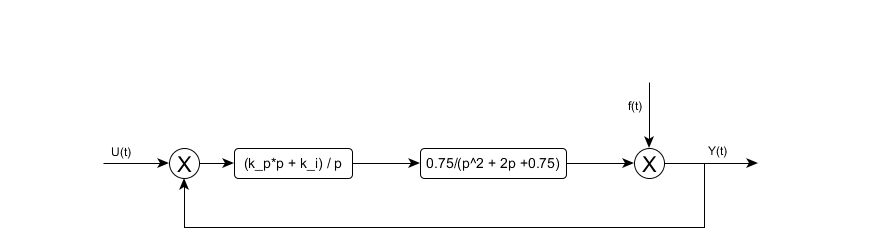
\includegraphics[scale = 0.55]{images/w.png}
	\caption{Структурная схема системы}
	\label{image:1}
\end{figure}

\FloatBarrier
Определим передаточную функцию разомкнутой системы:

$W_p=\frac{k_pp+k_i}{p}\frac{0.75}{p^2 + 2p + 0.75}  =\frac{0.75(k_pp+k_i)}{p(p^2 + 2p + 0.75)}$

Определим характеристический полином замкнутой системы:

$D(p)=B(p)+C(p)=p(p^2 + 2p + 0.75)+0.75(k_pp+k_i)=0.75k_i + 0.75(1 + k_p)p + 2p^2 + p^3$

Определим передаточную функцию замкнутой системы:

$W_3=\frac{W_p}{1 + W_p}=\frac{B(p)}{B(p)+C(p)}=\frac{B(p)}{D(p)}=\frac{0.75(k_pp+k_i)}{Tp^3+(2T+1)p^2+(0.75T+0.75k+2)p+0.75} 
$
%$= \frac{3kp}{4Tp^3+4(2T+1)p^2+(3T+3k+8)p+3}$



\subsection{Статическая ошибка}

Для данной системы статическая ошибка вычисляется следующим образом:


$e=lim_{t\rightarrow\infty}\frac{U(t)}{1+W_p(t)}$

\noindentТак как система является астатической первого порядка, то $e \rightarrow 0$

\subsection{Корневые критерии качества}

Данная группа критериев применяется для оценки качества системы по корням характеристического полинома:



$D(p)=0.75k_i + 0.75(1 + k_p)p + 2p^2 + p^3$


\textbf{Оценка быстродействия} может производиться на основе величины:


$\Omega=\sqrt[n]{|p_1\cdot...\cdot p_n|}$


Для данной системы существует три корня:

$\Omega=\sqrt[3]{|p_1\cdot p_2\cdot p_3|}=\sqrt[3]{-0.75k_i}$
Видно, что система достигнет наилучшего быстродействия при значении $k_i = 0$.

\textbf{Степень устойчивости} системы определяется как абсолютное значение действительной части корней, ближайших к мнимой оси корня (к нулю):

$realPart = min(|Re(p_1)|, |Re(p_2)|, |Re(p_3)|)$

Таким образом, для получения оптимальных параметров $k_i$ и $k_P$, значение $realPart$ нужно минимизировать. В результате минимизации получились значения $k_i = 0$ и $k_p = 100$. 
Значения корней при полученных значениях параметров:

$\begin{cases}
 p_1 = 0\\p_2 = -1 + 8j\\ p_3 = -1 -8j 
 \end{cases}
 $

\textbf{Колебательность системы} определяется мнимыми частями корней. Для нулевой колебательности все мнимые части корней должны быть равны нулю.
Таким образом, для получения оптимальных параметров $k_i$ и $k_p$, должно быть выполнено условие:

$\begin{cases}
Imagine(p_1)=0\\Imagine(p_2)=0\\Imagine(p_3)=0
\end{cases}
$

Так как условие не выполняется, можно сказать, что при полученных значениях параметров
в системе имеется колебательность.



\subsection{Анализ полученной системы}


Эксперементально было выяснено, что оптимальное значение  $k = 0.04$ и $T = 35$.
Cтатическая ошибка: $e = 0$ 
Корни характеристического уравнения:

$\begin{cases}
 p_1 = 0.0133\\p_2 =0.0133\\ p_3 =-0.0267
 \end{cases}
 $
 

\begin{figure}[h!]
	\centering
	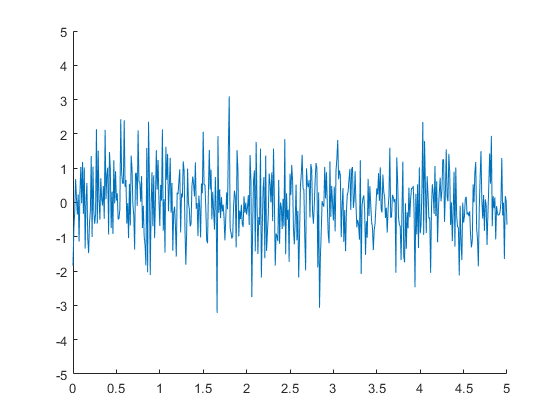
\includegraphics[scale = 0.80]{images/noise.png}
	\caption{Шум накладываемый на переходную характеристику}
	\label{image:9}
\end{figure}

\FloatBarrier


\begin{figure}[h!]
	\centering
	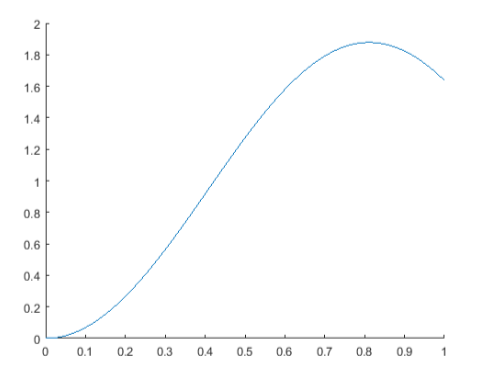
\includegraphics[scale = 0.80]{images/wnoise.png}
	\caption{Переходная характеристика без наложения шума}
	\label{image:9}
\end{figure}
\FloatBarrier

\begin{figure}[h!]
	\centering
	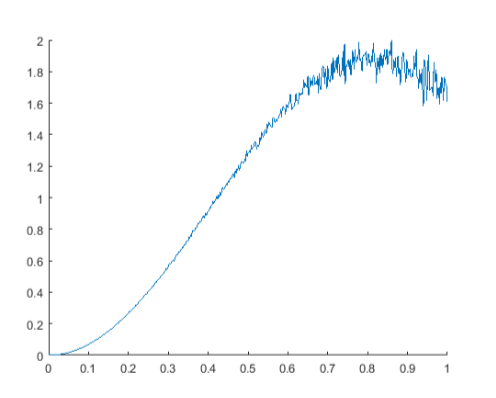
\includegraphics[scale = 0.80]{images/1.png}
	\caption{Переходная характеристика с наложением шума}
	\label{image:9}
\end{figure}
\FloatBarrier


Видно, что в промежуток времени, когда значение выходного сигнала возрастает, наличие шума практически не сказывается на поведении системы. Наибольшее
влияние обнаруживается, когда после этого система устремляется к значению в установившемся режиме. Также на графике видна колебательность системы.

\section{Вывод}

Анализ зависимости характеристик качества от параметров системы показал, что для исследуемой системы установить оптимальные параметры однозначно. Любые отклонения, в большую или меньшую сторону ухудшают качественные характеристики ситсемы и вносят элемент колебательности. 

По значениям корней можно сделать вывод, что система находится на апериодической границе
устойчивости. Также можно сказать, что в системе присутствует колебательность. Это
подтверждается результатами на графике.


\end{document}
